% SENTINEL-E: Anytime-Valid Sequential Detection for Streaming Illegal Dumping
% Surveillance.  Prepared for the Neural Computing and Applications topical
% collection "Emerging Trends in Smart Waste Monitoring and Environmental
% Surveillance".  For submission, replace the preamble with Springer's
% sn-jnl.cls; the body is class-independent.
\documentclass[11pt,a4paper]{article}

\usepackage[T1]{fontenc}
\usepackage[utf8]{inputenc}
\usepackage{lmodern}
\usepackage[margin=2.5cm]{geometry}
\usepackage{amsmath,amssymb,amsthm}
\usepackage{graphicx}
\usepackage{booktabs}
\usepackage{pifont}
\usepackage{caption}
\usepackage{subcaption}
\usepackage{microtype}
\PassOptionsToPackage{hidelinks}{hyperref}
\usepackage{hyperref}
\usepackage{orcidlink}
\usepackage[capitalise,noabbrev]{cleveref}
\usepackage{natbib}
\bibliographystyle{plainnat}

\graphicspath{{../results/figures/}}
% Auto-generated by experiments/make_macros.py -- do not edit.
% Every number quoted in the manuscript prose is defined here and comes
% directly from the JSON payloads written by the experiment scripts.

\newcommand{\ExpOneHorizonReps}{200}
\newcommand{\ExpOneReps}{1500}
\newcommand{\HorizonFixedPfa}{1.000}
\newcommand{\HorizonFixedPfaPct}{100}
\newcommand{\HorizonFixedPfaShort}{0.640}
\newcommand{\HorizonMaxFrames}{240{,}000}
\newcommand{\HorizonMaxHours}{2.7}
\newcommand{\HorizonMinHours}{0.2}
\newcommand{\HorizonPvaluePfa}{1.000}
\newcommand{\HorizonPvaluePfaPct}{100}
\newcommand{\HorizonSentinelPfa}{0.000}
\newcommand{\ValidityAlphaLoose}{0.20}
\newcommand{\ValidityMaxSentinelPfa}{0.001}
\newcommand{\ValidityPfaOracleLoose}{0.044}
\newcommand{\ValidityPfaPvalue}{0.998}
\newcommand{\ValidityPfaPvaluePct}{100}
\newcommand{\ValidityPfaSentinel}{0.000}
\newcommand{\ValidityPvalueArl}{11{,}155}
\newcommand{\ValidityPvalueArlMin}{7.4}
\newcommand{\ValidityTightestAlpha}{0.005}
\newcommand{\ValidityTightestCiHi}{0.003}
\newcommand{\ValidityTightestPfa}{0.000}
\newcommand{\ValidityWorstCiHi}{0.004}

% Placeholders for experiments that have not been run yet.  These make
% the manuscript compile from a partial results directory; a '??' in the
% PDF means the corresponding experiment output is missing.
\providecommand{\AblChangepointDelay}{\textbf{??}}
\providecommand{\AblChangepointMiss}{\textbf{??}}
\providecommand{\AblChangepointPfa}{\textbf{??}}
\providecommand{\AblDilationDelay}{\textbf{??}}
\providecommand{\AblDkwDelay}{\textbf{??}}
\providecommand{\AblDkwSpeedup}{\textbf{??}}
\providecommand{\AblEveryFramePfa}{\textbf{??}}
\providecommand{\AblFullDelay}{\textbf{??}}
\providecommand{\AblFullMiss}{\textbf{??}}
\providecommand{\AblLag}{\textbf{??}}
\providecommand{\AblNoCcPfa}{\textbf{??}}
\providecommand{\AblNumInvalid}{\textbf{??}}
\providecommand{\AblNumVariants}{\textbf{??}}
\providecommand{\AblPointPriorMiss}{\textbf{??}}
\providecommand{\AblPooledPfa}{\textbf{??}}
\providecommand{\AblRawCalPfa}{\textbf{??}}
\providecommand{\CostBackboneMs}{\textbf{??}}
\providecommand{\CostBackboneParams}{\textbf{??}}
\providecommand{\CostFitSec}{\textbf{??}}
\providecommand{\CostRealtimeFactor}{\textbf{??}}
\providecommand{\CostSentinelPct}{\textbf{??}}
\providecommand{\CostSentinelUs}{\textbf{??}}
\providecommand{\CoverDaytimeAbstain}{\textbf{??}}
\providecommand{\CoverDaytimeMiss}{\textbf{??}}
\providecommand{\DelayInadmissibleList}{\textbf{??}}
\providecommand{\DelayNumInadmissible}{\textbf{??}}
\providecommand{\DelaySentinelCi}{\textbf{??}}
\providecommand{\DelaySentinelMiss}{\textbf{??}}
\providecommand{\DelaySentinelPfa}{\textbf{??}}
\providecommand{\DelaySentinelSec}{\textbf{??}}
\providecommand{\DiagAcfRaw}{\textbf{??}}
\providecommand{\DiagAcfThin}{\textbf{??}}
\providecommand{\DiagLjungRaw}{\textbf{??}}
\providecommand{\DiagLjungThin}{\textbf{??}}
\providecommand{\DiagPmin}{\textbf{??}}
\providecommand{\EpiHardPiCpMiss}{\textbf{??}}
\providecommand{\EpiHardPiEpiMiss}{\textbf{??}}
\providecommand{\EpiManyCpDelay}{\textbf{??}}
\providecommand{\EpiManyCpMiss}{\textbf{??}}
\providecommand{\EpiManyEpiDelay}{\textbf{??}}
\providecommand{\EpiManyEpiMiss}{\textbf{??}}
\providecommand{\EpiMaxCount}{\textbf{??}}
\providecommand{\EpiMinPi}{\textbf{??}}
\providecommand{\EpiOneCpDelay}{\textbf{??}}
\providecommand{\EpiOneCpMiss}{\textbf{??}}
\providecommand{\EpiOneEpiDelay}{\textbf{??}}
\providecommand{\EpiOneEpiMiss}{\textbf{??}}
\providecommand{\ExpTwoReps}{\textbf{??}}
\providecommand{\NetCameras}{\textbf{??}}
\providecommand{\NetFdrLevel}{\textbf{??}}
\providecommand{\NetFleets}{\textbf{??}}
\providecommand{\NetGnnDelayReduction}{\textbf{??}}
\providecommand{\NetGnnDelaySec}{\textbf{??}}
\providecommand{\NetGnnFdr}{\textbf{??}}
\providecommand{\NetGnnNullPfa}{\textbf{??}}
\providecommand{\NetGnnPower}{\textbf{??}}
\providecommand{\NetNoGraphDelaySec}{\textbf{??}}
\providecommand{\NetNoGraphNullPfa}{\textbf{??}}
\providecommand{\ShiftMaxRatio}{\textbf{??}}
\providecommand{\ShiftMondrianPfa}{\textbf{??}}
\providecommand{\ShiftPooledPfa}{\textbf{??}}
\providecommand{\ShiftResidualPfa}{\textbf{??}}


\theoremstyle{plain}
\newtheorem{theorem}{Theorem}
\newtheorem{lemma}[theorem]{Lemma}
\newtheorem{proposition}[theorem]{Proposition}
\theoremstyle{definition}
\newtheorem{definition}[theorem]{Definition}
\newtheorem{remark}[theorem]{Remark}

\newcommand{\Pinf}{\mathbb{P}_{\infty}}
\newcommand{\Einf}{\mathbb{E}_{\infty}}
\newcommand{\Fcal}{\mathcal{F}}
\newcommand{\cD}{\mathcal{D}}
\newcommand{\ind}[1]{\mathbf{1}\{#1\}}
\newcommand{\ARL}{\mathrm{ARL}_0}
\newcommand{\ADD}{\mathrm{ADD}}
\newcommand{\PFA}{\mathrm{PFA}}

\title{\textbf{SENTINEL-E}: Anytime-Valid Sequential Detection for\\
       Streaming Illegal Dumping Surveillance}

\author{%
  Quang-Vinh Dang\,\orcidlink{0000-0002-3877-8024}\\[2pt]
  \small British University Vietnam, Hung Yen, Vietnam\\
  \small \texttt{vinh.dq4@buv.edu.vn}
}
\date{}

\begin{document}
\maketitle

\begin{abstract}
\noindent
Computer-vision systems for illegal dumping are trained and evaluated as
fixed-sample-size classifiers: given a short clip, emit one dumping /
no-dumping decision and report clip-level precision and recall. Deployment does
not look like that. A municipal camera runs for weeks, and the quantity an
operator actually manages is the number of false alarms accumulated over the
whole monitoring period, because each one costs an enforcement dispatch.
Applying a fixed threshold repeatedly to a continuous stream and alerting the
first time it is crossed is optional stopping, and it inflates the true
false-alarm rate by an amount clip-level evaluation cannot show. We measure the
effect and find it severe: a per-frame rule built on p-values that are
individually valid at the $1\%$ level raises at least one false alarm on
\ValidityPfaPvalue{} of $40$-minute null streams, and on \HorizonPvaluePfa{} of
\HorizonMaxHours-hour streams.
%
We introduce SENTINEL-E, a three-layer wrapper that converts any frozen
per-frame dumping detector into a network of anytime-valid sequential detectors
with time-uniform false-alarm control. Raw scores become conformal p-values
against a per-camera set of confirmed no-dumping frames, calibrated
conditionally on observable context and corrected by exact Beta order-statistic
levels that are an order of magnitude tighter in the tail than the usual
concentration bound. Each camera then runs a betting e-detector whose wealth is
a non-negative supermartingale under the no-dumping null, so thresholding at
$1/\alpha$ controls the false-alarm probability \emph{simultaneously at every
frame}, with no penalty for monitoring longer. Finally, cameras are organised
into a graph whose neural spatial prior steers the bets through a
\emph{predictable} hazard and stake modulation --- provably unable to damage the
guarantee, whatever it outputs --- and fleet decisions are combined by e-BH,
which controls the false-discovery rate under arbitrary dependence.
%
Across \ExpTwoReps{} Monte-Carlo streams per operating point, SENTINEL-E is the
only method examined whose realised false-alarm rate stays at or below its
nominal level at every setting, while detecting events in
\DelaySentinelSec\,s. Of the components ablated, the ones that turn out to be
load-bearing for validity are temporal decorrelation and conditional
calibration, not the betting or prior choices. Because the guarantee layer sits
on a frozen backbone and its per-frame arithmetic is $O(1)$, it costs
\CostSentinelUs\,\textmu s per frame --- \CostSentinelPct\% of the detector it
wraps --- and is therefore deployable on edge hardware that already runs the
detector in real time.
\end{abstract}

\vspace{0.5em}
\noindent\textbf{Keywords:} illegal dumping detection; anytime-valid inference;
e-values; conformal prediction; sequential change detection; false discovery
rate; video surveillance; edge deployment

\section{Introduction}
\label{sec:intro}

Illegal dumping is a persistent municipal problem with an obvious
computer-vision framing, and the field has adopted that framing consistently:
collect clips, label them as containing a dumping event or not, train a video
classifier, report clip-level accuracy. The recent release of Mivia-IWDD-500
\citep{greco2026iwdd} --- the first public dataset for illegal waste dumping
detection, with $250$ positive and $250$ negative surveillance videos and
onset timestamps --- gives the field a shared benchmark on exactly these terms,
and the reference baseline distributed with it is evaluated on exactly these
terms.

The framing does not match deployment. A camera watching a lay-by does not
receive a curated ten-second clip and return a verdict; it produces frames
continuously for weeks, and the system alerts the first time its evidence
crosses some threshold. What the municipality manages is not per-clip precision
but the number of enforcement dispatches wasted over a season. Those two
quantities are related by a step that the clip-level protocol never exercises:
\emph{repeatedly} testing a stream and stopping at the first exceedance is
optional stopping, and it invalidates the level at which any fixed threshold
was calibrated.

The magnitude of the gap is easy to state and, we find, easy to underestimate.
A rule that raises a false alarm on each frame with probability $q$ raises at
least one over $T$ frames with probability $1-(1-q)^{T}$, which tends to one for
any $q>0$. Persistence filters and score smoothing change $q$; they do not
change the limit. Our measurements bear this out. Feeding a per-frame rule
p-values that are individually and provably valid at the $1\%$ level --- so that
nothing is wrong with the calibration --- produces at least one false alarm on
\ValidityPfaPvalue{} of $40$-minute null streams
(\cref{fig:validity}\,(a)); a raw score threshold tuned to a $10^{-3}$ per-frame
rate reaches \HorizonFixedPfaShort{} within \HorizonMinHours\,hours and
\HorizonFixedPfa{} by \HorizonMaxHours\,hours (\cref{fig:validity}\,(b)). None
of this is visible in a clip-level evaluation, because a clip-level evaluation
never runs the detector for two hours.

The tools that solve exactly this problem are mature. Ville's inequality
\citep{ville1939} bounds the probability that a non-negative supermartingale
\emph{ever} exceeds a level, and the modern game-theoretic literature
\citep{shafer2019game,ramdas2023savi,grunwald2024evalues} has turned that into a
practical construction: bet against the null, and the accumulated wealth is a
time-uniform certificate. Conformal prediction \citep{vovk2005alrw} supplies
distribution-free p-values, e-detectors \citep{shin2024edetectors} adapt the
machinery to change detection, and e-BH \citep{wang2022ebh} combines evidence
across many streams under arbitrary dependence. To our knowledge none of it has
been applied to waste, dumping or pollution surveillance. We think that gap is
not a coincidence but a consequence of the clip-level framing: a protocol that
never runs a detector continuously never surfaces the problem these tools
solve.

Closing it is not a matter of importing the machinery unchanged. Surveillance
streams violate the assumptions three times over, and each violation is fatal
in a way that only shows up when the guarantee is actually measured rather than
cited.

\begin{enumerate}
\item \textbf{The frame rate is not the evidence rate.} Consecutive frames of
      video are near-duplicates, so backbone scores are strongly
      autocorrelated. Every sequential test assumes conditionally independent
      increments. Betting on each of $25$ frames per second inflates a nominal
      $\alpha=0.01$ to a realised \AblEveryFramePfa{} in our experiments --- the
      single most damaging mistake we found, and one invisible in the algebra.
\item \textbf{Marginal calibration is not conditional calibration.} A
      night-time score compared against a calibration set dominated by daylight
      is marginally valid and locally useless: during the hours when the
      backbone runs hot, its p-values are systematically too small, and a
      sequential test converts that local miscalibration into an early alarm.
      Pooled conformal calibration gives a realised \AblPooledPfa{} at a
      nominal $0.01$.
\item \textbf{The calibration set is finite and gets reused forever.}
      Conditional on it --- which is the only conditioning that matters, since
      the same set scores every frame for months --- the p-values are only
      approximately uniform, by $O(n^{-1/2})$. Ignoring this gives a realised
      \AblNoCcPfa{}. Correcting it with the standard
      Dvoretzky--Kiefer--Wolfowitz inflation restores validity but is
      catastrophically loose in the tail, which is where a betting detector
      earns its wealth.
\end{enumerate}

\subsection{Contributions}

\begin{itemize}
\item \textbf{A formulation of dumping surveillance as anytime-valid sequential
      detection}, with the operational metrics that follow from it --- delay at
      a controlled false-alarm rate over a monitoring horizon --- and a protocol
      that converts any clip-labelled corpus into long streams without new data
      collection (\cref{sec:problem}).

\item \textbf{Exact calibration-conditional conformal levels.}
      Rather than inflating p-values additively, we replace each attainable
      level by its exact Beta order-statistic upper confidence bound
      (\cref{thm:beta}). At $n=2000$ and $\delta=10^{-3}$ this puts the smallest
      usable p-value at $0.0037$ instead of the $0.051$ that DKW permits, a
      $14\times$ improvement precisely where the evidence is. In the ablation it
      is worth a factor of \AblDkwDelay/\AblFullDelay{} in detection delay
      (\cref{sec:ablation}).

\item \textbf{A changepoint-mixture e-process that is an exact supermartingale.}
      Retaining the not-yet-reached prior mass inside the statistic
      (\cref{sec:layer2}) upgrades the classical Shiryaev--Roberts average-run-length
      bound to a time-uniform probability bound, at a cost logarithmic in the
      horizon, and collapses to an $O(1)$ recursion.

\item \textbf{A learned spatial prior that provably cannot break the
      guarantee.} A graph network steers each camera's hazard and stake from its
      neighbours' wealth. Because the modulation is predictable, the wealth
      remains a supermartingale whatever the network outputs
      (\cref{thm:predictable}) --- so a learned component sits on top of a formal
      guarantee with none of the usual caveats. Fleet decisions use e-BH, valid
      under the dependence the graph deliberately induces.

\item \textbf{An evaluation that measures guarantees instead of asserting
      them}, over \ExpOneReps{} Monte-Carlo streams per operating point,
      against five baselines including a reimplementation of the closest
      generic prior art \citep{khan2026eshift}; a component ablation in which
      \AblNumInvalid{} of \AblNumVariants{} variants fail to deliver the level
      they claim; and a cost measurement showing the guarantee layer runs at
      \CostSentinelPct\% of its backbone.
\end{itemize}

We are explicit about scope in \cref{sec:limitations}: the streaming results are
obtained on a score-level simulator calibrated to plausible backbone behaviour,
because no released corpus provides the months of continuously-labelled
per-frame detector output that a time-uniform claim must be tested against, and
we did not have access to one. The library ships adapters and a splicing
protocol so the same evaluation runs on Mivia-IWDD and the other corpora as soon
as backbone scores are available, and no adapter fabricates data when they are
not.

\section{Related work}
\label{sec:related}

\paragraph{Waste and dumping detection.}
Image-level litter detection is well served by TACO \citep{proenca2020taco} and
ZeroWaste \citep{bashkirova2022zerowaste}; UAV and wide-area monitoring by
UAVVaste \citep{kraft2021uavvaste} and AerialWaste
\citep{torres2023aerialwaste}; marine pollution by MARIDA
\citep{kikaki2022marida} and MADOS \citep{kikaki2024mados}. Video-based dumping
detection has, until recently, lacked a public benchmark; Mivia-IWDD-500
\citep{greco2026iwdd} supplies one together with a reference baseline. All of
these are evaluated per image or per clip. We are not aware of any work in this
literature that reports a false-alarm rate over a monitoring horizon, which is
the quantity a deployment is judged by, nor any that addresses optional
stopping. SENTINEL-E is complementary rather than competing: it consumes a
frozen backbone's scores and adds a guarantee layer, so a better backbone and
this work compound.

\paragraph{Sequential change detection.}
CUSUM \citep{page1954}, Shiryaev's Bayesian statistic \citep{shiryaev1963} and
Shiryaev--Roberts \citep{roberts1966} are the classical procedures, with
optimality theory due to \citet{lorden1971} and \citet{moustakides1986}. Their
guarantees are asymptotic average-run-length statements that presume a correctly
specified pre-change law. Detector scores from real footage are autocorrelated,
heavy-tailed and diurnally non-stationary, so the presumption fails; both
baselines lose control in our experiments. \citet{shin2024edetectors} give a
nonparametric e-detector framework with clean non-asymptotic ARL bounds, which
is the closest ancestor of our Layer 2. We depart from it in retaining the
unreached changepoint prior mass, which converts the ARL bound into a
time-uniform probability bound.

\paragraph{Anytime-valid inference and e-values.}
Testing by betting \citep{shafer2021testing,ramdas2023savi,grunwald2024evalues}
turns Ville's inequality into a design principle; \citet{waudby2024betting}
develop the betting strategies we adapt. \citet{wang2022ebh} introduce e-BH,
which controls FDR under arbitrary dependence and underpins our fleet layer;
\citet{vovk2021evalues} characterise e-value merging. Closest to this work in
spirit is E-SHIFT \citep{khan2026eshift}, which detects distribution shift in
streaming learning systems with a sub-Gaussian e-process built on a composite
non-conformity score. We reimplement it as a baseline. It differs from
SENTINEL-E in three ways that matter here: its log-moment-generating-function
bound is estimated, so validity is asymptotic in the calibration size rather
than finite-sample; it assumes unconditional exchangeability with calibration,
which a diurnal cycle breaks; and its wealth starts at frame one, so evidence
arriving hours into a stream must first repay what was burned before it.

\paragraph{Conformal prediction.}
Split conformal prediction \citep{vovk2005alrw} supplies the distribution-free
p-values we bet on. \citet{vovk2012conditional} studies calibration-conditional
validity, which is the concern our Beta levels address, and
\citet{tibshirani2019covariate} handle covariate shift by likelihood-ratio
weighting, which we implement and evaluate. Conformalising a normalised
regression residual is standard practice
\citep{lei2018distribution,romano2019cqr}, and localisation
\citep{guan2023localized} pursues conditional coverage by other means. Our Layer
1 combines these with the sequential requirement, which imposes a constraint the
prediction-interval literature does not face: the p-values must be
super-uniform \emph{conditionally on the past}, not merely marginally, or the
wealth process is not a supermartingale.

\section{Problem formulation}
\label{sec:problem}

A camera produces frames $x_1, x_2, \ldots$ and a frozen detector
$g$ produces scores $s_t = g(x_t) \in \mathbb{R}$, with higher meaning more
dumping-like. Alongside each frame we observe a low-dimensional context vector
$c_t \in \mathbb{R}^d$ --- time of day, a weather flag, ambient luminance, a
background-subtraction motion measure --- available to any deployed camera
without privileged knowledge. The operator supplies a per-camera calibration set
$\cD = \{(s_i^{\mathrm{cal}}, c_i^{\mathrm{cal}})\}_{i=1}^{n}$ of confirmed
no-dumping frames.

Write $\Pinf$ for the law of the stream under ``no dumping ever'' and
$\mathbb{P}_{\nu}$ for the law when dumping begins at frame $\nu$. A detection
rule is a stopping time $\tau$ with respect to the observation filtration
$(\Fcal_t)$. We require:

\begin{definition}[Time-uniform false-alarm control]
\label{def:tuv}
A rule has time-uniform false-alarm level $\alpha$ if
$\Pinf(\tau < \infty) \le \alpha$.
\end{definition}

The quantifier is the whole point. A per-frame guarantee
$\Pinf(\text{alarm at } t) \le \alpha$ for each fixed $t$ says nothing about
$\Pinf(\exists t : \text{alarm at } t)$, and the gap between them grows with the
horizon. \Cref{def:tuv} is what a municipality is implicitly buying when it is
told a detector has a $1\%$ false-alarm rate.

We report, over Monte-Carlo replicates:
$\PFA$, the probability that a null stream of a stated length raises at least
one alarm; $\ARL$, the mean frames to a false alarm on a null stream, censored
at the horizon; $\ADD$, the mean frames from onset $\nu$ to the first alarm at
or after it, over runs that alarm; and the miss rate, the fraction of
post-change segments that end unflagged. Every comparison is made at a method's
\emph{realised} $\PFA$, never its nominal one, since a method whose nominal
level is meaningless would otherwise appear to dominate by misreporting its own
error rate.

\paragraph{From clips to streams.}
A clip-labelled corpus such as Mivia-IWDD becomes a streaming benchmark without
new data collection. Reserve a disjoint subset of confirmed-negative clips as
$\cD$; concatenate the remaining negative clips into a background stream of the
desired length; splice positive clips in at random onsets. Holding the
calibration clips out preserves the exchangeability the conformal layer needs.
This protocol is implemented in the library
(\texttt{build\_stream\_from\_clips}) and is how we recommend the method be
evaluated once per-frame backbone scores for a real corpus are in hand.

\section{Method}
\label{sec:method}

\subsection{Layer 1: conformal calibration}
\label{sec:layer1}

\paragraph{Betting rate.}
The e-process of \cref{sec:layer2} requires increments that are conditionally
super-uniform given the past. Video violates this badly: at $25$\,fps the
lag-one autocorrelation of backbone scores exceeds $0.85$ in our streams. We
estimate a decorrelation lag $\ell$ from the calibration set alone --- projecting
out the context-predictable drift first with a quadratic least-squares fit, since
otherwise the slow diurnal component dominates the autocorrelation and returns a
uselessly large $\ell$ --- and place one bet per $\ell$ frames. In our streams
$\ell = \AblLag$, so bets occur more than once per second, far finer than the
timescale of a dumping event. The same reasoning applies to the calibration
frames, which are consecutive video too: they are thinned by $\ell$ before use,
so the honest calibration size is $n/\ell$ and it is that number the guarantee is
stated in. \Cref{sec:ablation} shows this is not a refinement: betting on every
frame is the single largest source of invalidity we measured.

\paragraph{Conditional calibration.}
Let $S$ be a nonconformity score. The split-conformal p-value of a deployment
frame is $p = (1 + |\{i : S_i \ge S\}|)/(n+1)$, which is super-uniform under
exchangeability. Exchangeability between a night-time frame and a
daylight-dominated $\cD$ is exactly what fails. We therefore conformalise the
\emph{context-normalised residual}
\begin{equation}
\label{eq:residual}
  z \;=\; \frac{s - \hat g(c)}{\hat\sigma(c)},
  \qquad
  \hat g(c) \approx \mathbb{E}[s \mid c],
  \quad
  \hat\sigma(c) \approx \mathbb{E}\bigl[|s - \hat g(c)| \,\big|\, c\bigr],
\end{equation}
with $\hat g$ and $\hat\sigma$ ridge regressions on a quadratic-with-interactions
basis in $c$, fitted on one half of $\cD$ and conformalised on the other. The
split preserves exchangeability between calibration and deployment residuals
exactly, and the whole held-out half backs every context value --- unlike
Mondrian binning, where a bin's worth must cover each one. We implement Mondrian
calibration as well, since it is exactly group-conditional and preferable when a
single context variable dominates; \cref{sec:shift} shows where each wins.

Because a regression can be extrapolated but a guarantee cannot, frames whose
context falls outside the region $\cD$ covers --- a per-coordinate box widened by
a margin, intersected with a Mahalanobis check for jointly novel combinations ---
are reported inactive, and the detector bets neutrally on them. A regime that was
never calibrated cannot be certified, and the abstention rate reports how often
that happens rather than hiding it.

\paragraph{Calibration-conditional validity.}
The same finite $\cD$ scores every frame for months, so the relevant statement is
conditional on $\cD$, and conditionally the p-values deviate from uniform by
$O(n^{-1/2})$. The standard remedy adds the Dvoretzky--Kiefer--Wolfowitz
deviation $\varepsilon_n(\delta) = \sqrt{\log(2/\delta)/(2n)}$
\citep{dkw1956,massart1990} to every p-value. It works and it is far too blunt:
at $n=2000$, $\delta=10^{-3}$ it moves the smallest attainable p-value from
$1/2001$ to $0.051$, capping the evidence a single frame can supply at well under
one nat. The tail is the only part a betting detector uses.

We use the exact distribution instead.

\begin{theorem}[Exact calibration-conditional levels]
\label{thm:beta}
Let $S_1,\dots,S_n$ be i.i.d.\ from a continuous $F$ and let $S$ be an
independent draw from $F$. For $j = 0,\dots,n-1$ let $\delta_j > 0$ with
$\sum_j \delta_j \le \delta$, and set
\begin{equation}
\label{eq:betalevels}
  q_j \;=\; \mathrm{Beta}^{-1}\bigl(1-\delta_j;\; j+1,\; n-j\bigr),
  \qquad q_n = 1 .
\end{equation}
Define $\tilde p = q_{J}$ with $J = |\{i : S_i \ge S\}|$. Then there is an event
$E$ with $\mathbb{P}(E) \ge 1-\delta$, measurable with respect to
$S_1,\dots,S_n$, on which
$\mathbb{P}\bigl(\tilde p \le u \mid S_1,\dots,S_n\bigr) \le u$
for every $u \in [0,1]$.
\end{theorem}

\begin{proof}
Conditionally on the calibration sample, $\{J \le j\} = \{S > S_{(n-j)}\}$ where
$S_{(1)} \le \cdots \le S_{(n)}$ are the order statistics, so
$\mathbb{P}(J \le j \mid \cD) = 1 - F(S_{(n-j)})$. Since $F$ is continuous,
$F(S_{(k)}) \sim \mathrm{Beta}(k, n+1-k)$, hence
$1 - F(S_{(n-j)}) \sim \mathrm{Beta}(j+1, n-j)$. By \cref{eq:betalevels},
$\mathbb{P}\bigl(1 - F(S_{(n-j)}) > q_j\bigr) = \delta_j$. Let $E$ be the
intersection over $j$ of the complements; a union bound gives
$\mathbb{P}(E) \ge 1 - \sum_j \delta_j \ge 1-\delta$. On $E$,
$\mathbb{P}(\tilde p \le q_j \mid \cD) = \mathbb{P}(J \le j \mid \cD) \le q_j$
for every $j$, and since $\tilde p$ takes values only in $\{q_0,\dots,q_n\}$
and $q_j$ is non-decreasing in $j$, super-uniformity at the atoms extends to all
$u$.
\end{proof}

We spend the budget as $\delta_j \propto (j+1)^{-2}$, concentrating confidence
where the betting functions look. At $n=2000$, $\delta=10^{-3}$ this gives
$q_0 = 0.0037$ against DKW's $0.051$. \Cref{thm:beta} assumes i.i.d.\ calibration
draws, which is why the calibration set is thinned; the ablation confirms that
skipping the thinning costs validity.

Finally, when deployment reweights context that $\cD$ does cover, weighted
conformal calibration \citep{tibshirani2019covariate} applies. We implement it
with a logistic density-ratio estimate, gate it behind a held-out
classifier two-sample test so it engages only when a shift is detectable, and
take the calibration-conditional correction at the Kish effective sample size
\citep{kish1965}. \Cref{sec:shift} reports that in our setting the residual
construction of \cref{eq:residual} dominates it, which we take to be a fact about
the setting rather than about the technique: reweighting corrects the marginal
context distribution, while a sequential test is broken by \emph{conditional}
miscalibration.

\subsection{Layer 2: the betting e-detector}
\label{sec:layer2}

Let $p_1, p_2, \ldots$ be the p-values at the betting instants. A
\emph{betting function} is a non-increasing $f : (0,1] \to [0,\infty)$ with
$\int_0^1 f \le 1$; then $\mathbb{E}_{H_0}[f(p)] \le 1$ for any super-uniform
$p$, so $f(p)$ is an e-value. We use the power family
$f_\kappa(p) = \kappa p^{\kappa-1}$, $\kappa \in (0,1]$, mixed over a
log-spaced grid; $\kappa = 1$ gives the neutral bet $f \equiv 1$.

Dumping begins at an unknown $\nu$. Place a prior $w_1, w_2, \ldots$ with
$\sum_j w_j = 1$ on it and define
\begin{equation}
\label{eq:wealth}
  W_t \;=\;
  \underbrace{\sum_{j \le t} w_j \prod_{s=j}^{t} f(p_s)}_{R_t}
  \;+\;
  \underbrace{\sum_{j > t} w_j}_{Q_t} .
\end{equation}

\begin{theorem}[Time-uniform validity]
\label{thm:ville}
Under $\Pinf$, if the $p_t$ are conditionally super-uniform given $\Fcal_{t-1}$,
then $(W_t)$ is a non-negative supermartingale with $W_0 = 1$, and
\begin{equation*}
  \Pinf\bigl(\exists\, t \ge 1 : W_t \ge 1/\alpha\bigr) \;\le\; \alpha .
\end{equation*}
\end{theorem}

\begin{proof}
$W_0 = \sum_j w_j = 1$ and $W_t \ge 0$. Splitting off the term reached at $t$,
\begin{align*}
  \mathbb{E}[W_t \mid \Fcal_{t-1}]
   &= \Bigl(\textstyle\sum_{j \le t-1} w_j \prod_{s=j}^{t-1} f(p_s) + w_t\Bigr)
      \,\mathbb{E}[f(p_t) \mid \Fcal_{t-1}] \;+\; Q_t \\
   &\le R_{t-1} + w_t + Q_t \;=\; R_{t-1} + Q_{t-1} \;=\; W_{t-1},
\end{align*}
using $\mathbb{E}[f(p_t)\mid\Fcal_{t-1}] \le 1$ and $Q_{t-1} = Q_t + w_t$.
Ville's inequality \citep{ville1939} gives the bound.
\end{proof}

\begin{remark}
Dropping $Q_t$ from \cref{eq:wealth} recovers the Shiryaev--Roberts statistic,
which is \emph{not} a supermartingale --- the telescoping in the proof fails by
exactly $w_t$ per step --- and admits only an average-run-length bound. Carrying
the unreached prior mass is what buys \cref{def:tuv}. Its cost is
$-\log w_\nu \approx \log(1/\rho) + \nu\log(1/(1-\rho))$ nats of wealth to repay,
i.e.\ $O(\log T)$ for a hazard $\rho \sim 1/T$ matched to the horizon: the price
of monitoring $T$ frames grows logarithmically, against a fixed threshold whose
false-alarm probability grows to one.
\end{remark}

Writing $w_t = \rho_t Q_{t-1}$ and $Q_t = (1-\rho_t)Q_{t-1}$ keeps
$Q_{t-1} = Q_t + w_t$ exact even for a time-varying hazard, and \cref{eq:wealth}
collapses to
\begin{equation}
\label{eq:recursion}
  R_t = (R_{t-1} + w_t)\, f(p_t), \qquad Q_t = (1-\rho_t)\,Q_{t-1},
\end{equation}
evaluated in log space: $O(1)$ arithmetic and $O(K)$ memory for a $K$-point
mixture, independent of how long the camera has been running. For offline
evaluation the same recursion has the closed form
$R_t = P_t\bigl(R_0 + \sum_{j\le t} w_j / P_{j-1}\bigr)$ with
$P_t = \prod_{s\le t} f(p_s)$, which is one cumulative log-sum-exp and lets us
run the Monte-Carlo protocol at scale.

\subsection{Layer 3: the camera network}
\label{sec:layer3}

\paragraph{A predictable spatial prior.}
Offenders return to the same lay-by and, when disturbed, move a few hundred
metres and dump again, so evidence at one camera is genuine prior information
about its neighbours. We build a graph over the fleet with edge weights
combining spatial proximity and static-context similarity, and a two-layer
message-passing network maps each camera's features --- its own log-wealth, three
exponential moving averages of $-\log p$, static context and degree --- to a
hazard $\rho_{i,t}$ and a stake scale $m_{i,t}$, the latter interpolating the
power exponents towards the neutral bet, $\kappa_{\mathrm{eff}} = 1 - m(1-\kappa)$.

\begin{theorem}[Learned control cannot break the guarantee]
\label{thm:predictable}
Suppose $\rho_{i,t} \in [0,1]$ and $m_{i,t} \in [0,1]$ are $\Fcal_{t-1}$-measurable.
Then \cref{thm:ville} holds verbatim for every camera, for any such choice.
\end{theorem}

\begin{proof}
$\kappa_{\mathrm{eff}} = 1 - m_{i,t}(1-\kappa) \in (0,1]$ for any
$m_{i,t}\in[0,1]$, so $f_{\kappa_{\mathrm{eff}}}$ is a betting function and
$\mathbb{E}[f_{\kappa_{\mathrm{eff}}}(p_{i,t}) \mid \Fcal_{t-1}] \le 1$ because
$\kappa_{\mathrm{eff}}$ is $\Fcal_{t-1}$-measurable and may be taken outside the
conditional expectation. Likewise $w_t = \rho_{i,t} Q_{t-1}$ and
$Q_t = (1-\rho_{i,t})Q_{t-1}$ are $\Fcal_{t-1}$-measurable and satisfy
$Q_{t-1} = Q_t + w_t$ identically. The supermartingale step in \cref{thm:ville}
is therefore unchanged.
\end{proof}

This is worth stating plainly: the network can be badly trained, adversarially
initialised or handed the wrong topology, and the false-alarm guarantee still
holds. It can only affect detection delay. Training is offline on held-out
simulated fleets, maximising post-change log-wealth growth --- the Kelly / GROW
criterion \citep{kelly1956}, the standard proxy for minimising delay, since the
delay is essentially the time for the wealth to climb from one to $1/\alpha$ at
that rate --- with a penalty on wealth burned at unaffected cameras. The wealth
recursion is differentiable, so gradients reach both heads.

\paragraph{Fleet decisions.}
At a stopping time $\tau_i = \min(\text{first alarm}, T)$, optional stopping
gives $\Einf[W_{i,\tau_i}] \le 1$, so each camera's wealth is a valid e-value.
We apply e-BH \citep{wang2022ebh}: sort $E_{(1)} \ge \cdots \ge E_{(K)}$, reject
the top $k^\star = \max\{k : E_{(k)} \ge K/(\alpha k)\}$. This controls FDR at
$\alpha$ under \emph{arbitrary} dependence, which is what the setting demands:
adjacent cameras share weather, lighting and traffic, and Layer 3 couples them
deliberately. BH on p-values would need positive regression dependence or a
Benjamini--Yekutieli $\log K$ penalty \citep{benjamini2001}; e-BH needs neither.
A running maximum of the wealth would not be a valid e-value, which is why the
reading is taken at a stopping time.

\section{Experimental protocol}
\label{sec:protocol}

\paragraph{Streams.}
SENTINEL-E consumes one scalar per frame, so the faithful way to stress the
guarantee layer at the timescales that matter --- weeks of video, $10^6$ frames
--- is to model that scalar. Our simulator is deliberately unfriendly in the ways
real footage is: a diurnal illumination cycle and a two-state weather chain shift
the null score distribution after calibration; scores follow an AR(1) with
Student-$t$ innovations, so they are autocorrelated and heavy-tailed; a
log-scale Ornstein--Uhlenbeck scene-activity process drives the backbone's
false-positive rate and is deliberately \emph{not} part of the operator's obvious
(clock, weather) taxonomy; dumping events are intermittent, with only half the
frames in an event window anomalous and a ramp at each end; and events propagate
along the camera graph with a lag. Defaults put the null score near $0.24$ and
an anomalous frame near $0.75$, i.e.\ a per-frame signal weak enough that it
must accumulate over time --- the regime where sequential methods earn their
keep. \Cref{sec:limitations} states plainly what this does and does not
establish.

\paragraph{Baselines.}
A fixed score threshold with an optional $k$-of-$m$ persistence filter; a
per-frame threshold on the \emph{same} conformal p-values SENTINEL-E consumes,
which isolates optional stopping from calibration; CUSUM \citep{page1954};
Shiryaev--Roberts \citep{roberts1966}; a parametric e-detector using the same
changepoint mixture with a Gaussian likelihood-ratio bet instead of a conformal
one; and a reimplementation of E-SHIFT \citep{khan2026eshift}. Every baseline is
fitted on the same calibration set and evaluated on the same decorrelated
betting grid, so none is helped or penalised by the frame-rate choice. Each is
swept over its own knob and plotted at its realised false-alarm rate.

\paragraph{Reproducibility.}
Seeds are fixed in each script; \texttt{experiments/run\_all.py} reproduces every
number, and every quantity quoted in this text is generated into a macro file
from the experiment output, so a stale number is not possible. All timings are
single-thread CPU on the machine that produced the statistical results.

\section{Results}
\label{sec:results}

\subsection{False-alarm control is time-uniform}
\label{sec:validity}

\begin{figure}[t]
  \centering
  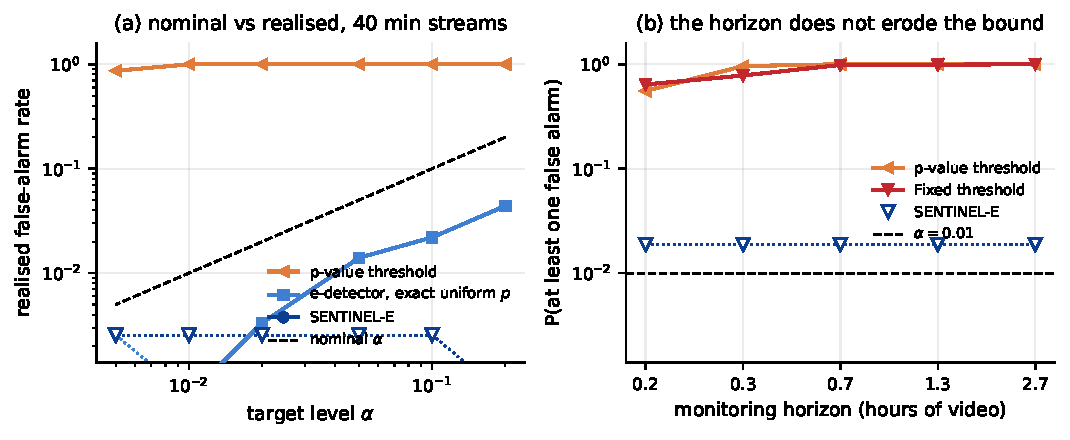
\includegraphics[width=\linewidth]{fig1_validity.pdf}
  \caption{Time-uniform false-alarm control, \ExpOneReps{} null streams per
  point. \textbf{(a)} Realised against nominal level. SENTINEL-E stays below the
  diagonal everywhere; the per-frame p-value threshold, fed \emph{identical}
  conformal p-values, sits at the top of the plot, so the difference is
  attributable to the stopping rule alone. The middle curve is the same
  e-detector fed exactly uniform p-values, which separates the slack in Ville's
  inequality from the conservatism of the conformal layer.
  \textbf{(b)} Against the monitoring horizon at $\alpha=0.01$. The per-frame
  rules approach one; SENTINEL-E is flat.}
  \label{fig:validity}
\end{figure}

\begin{table}[t]
\centering
\caption{Time-uniform false-alarm control on 40-minute null streams (300 Monte-Carlo streams per level). SENTINEL-E and the per-frame p-value threshold consume identical conformal p-values; only the stopping rule differs. ARL$_0$ is censored at the 60{,}000-frame horizon.}
\label{tab:validity}
\begin{tabular}{lrrrrrr}
\toprule
$\alpha$ & PFA & 95\% CI & PFA (oracle $p$) & ARL$_0$ & PFA & ARL$_0$ \\
\midrule
0.200 & 0.000 & [0.000, 0.013] & 0.037 & 60,000 & 1.000 & 105 \\
0.100 & 0.000 & [0.000, 0.013] & 0.007 & 60,000 & 1.000 & 257 \\
0.050 & 0.000 & [0.000, 0.013] & 0.000 & 60,000 & 1.000 & 598 \\
0.020 & 0.000 & [0.000, 0.013] & 0.000 & 60,000 & 1.000 & 2,764 \\
0.010 & 0.000 & [0.000, 0.013] & 0.000 & 60,000 & 1.000 & 12,239 \\
0.005 & 0.000 & [0.000, 0.013] & 0.000 & 60,000 & 0.853 & 29,114 \\
\bottomrule
\end{tabular}
\begin{minipage}{\linewidth}\vspace{2pt}\footnotesize Columns 2--3 and 5: SENTINEL-E; column 4 is the same e-detector fed exactly uniform p-values, isolating the slack in Ville's inequality from the conservatism of the conformal layer. Columns 6--7: per-frame p-value threshold. PFA is the probability that a null stream raises at least one alarm.\end{minipage}
\end{table}

\begin{table}[t]
\centering
\caption{False-alarm probability against monitoring horizon at $\alpha=0.01$ (fixed threshold calibrated to a $10^{-3}$ per-frame rate; 200 streams per point). SENTINEL-E is flat in the horizon; the per-frame rules are not.}
\label{tab:horizon}
\resizebox{\ifdim\width>\linewidth\linewidth\else\width\fi}{!}{%
\begin{tabular}{rrrrr}
\toprule
frames & hours & SENTINEL-E & p-value thr. & fixed thr. \\
\midrule
15,000 & 0.17 & 0.000 & 0.555 & 0.640 \\
30,000 & 0.33 & 0.000 & 0.960 & 0.780 \\
60,000 & 0.67 & 0.000 & 1.000 & 0.985 \\
120,000 & 1.33 & 0.000 & 1.000 & 0.990 \\
240,000 & 2.67 & 0.000 & 1.000 & 1.000 \\
\bottomrule
\end{tabular}}
\end{table}


\Cref{fig:validity} and \cref{tab:validity,tab:horizon} establish the basic
claim. At every level swept, SENTINEL-E's realised false-alarm probability is at
most \ValidityMaxSentinelPfa; the per-frame threshold on the same p-values
reaches \ValidityPfaPvalue{} at $\alpha=0.01$, with a mean of only
\ValidityPvalueArl{} frames to its first false alarm. Extending the horizon from
\HorizonMinHours{} to \HorizonMaxHours{} hours drives the p-value threshold to
\HorizonPvaluePfa{} and the fixed score threshold from \HorizonFixedPfaShort{} to
\HorizonFixedPfa, while SENTINEL-E remains at \HorizonSentinelPfa.

SENTINEL-E is conservative, and it is worth saying where the conservatism comes
from rather than presenting it as free. Feeding the same e-detector exactly
uniform p-values yields a realised \ValidityPfaOracleLoose{} at a nominal
\ValidityAlphaLoose: most of the gap is slack in Ville's inequality and in the
changepoint prior, not a cost of the conformal layer. Ville's bound is not tight,
and a practitioner who wants a realised rate close to nominal should calibrate
the threshold empirically; what the theory provides, and what a fixed threshold
cannot, is that the bound never degrades with the horizon.

\subsection{Detection delay at a controlled false-alarm rate}
\label{sec:delay}

\begin{figure}[t]
  \centering
  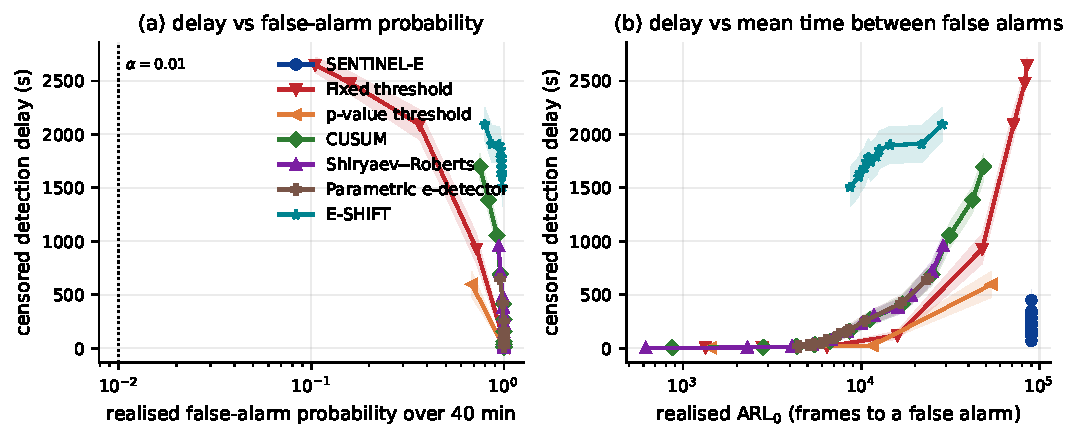
\includegraphics[width=\linewidth]{fig2_delay_far.pdf}
  \caption{Detection delay against realised false-alarm rate,
  \ExpTwoReps{} null and \ExpTwoReps{} post-change streams per operating point.
  Lower and further left is better; the operating region a municipality can live
  with is the left-hand edge. Each method is swept over its own knob and plotted
  where it actually lands, not where it claims to.}
  \label{fig:delayfar}
\end{figure}

\begin{table}[t]
\centering
\caption{Each method at the tightest realised false-alarm probability it achieves while still detecting most events, over a 60-minute stream (200 null and 200 post-change streams per operating point). This is the operator's question: insisting on few false alarms, what does the method cost in delay? Both exact e-processes tested (SENTINEL-E and the changepoint mixture it strictly contains, \cref{prop:generalisation}) reach a rate of at most 0.05; none of the classical or parametric baselines does. The classical procedures can be made fast, but only at a false-alarm probability near one for most settings of their knob; the full trade-off is in Figure~\ref{fig:delayfar}.}
\label{tab:delay_far}
\resizebox{\ifdim\width>\linewidth\linewidth\else\width\fi}{!}{%
\begin{tabular}{llrcrrrr}
\toprule
method & knob & realised PFA & $\le 0.05$? & ARL$_0$ & cond. delay (s) & censored delay (s) & miss rate \\
\midrule
SENTINEL-E & 0.5 & 0.000 & \checkmark & 90,000 & 54.6 & 68.3 $\pm$ 31.8 & 0.01 \\
Fixed threshold & $10^{-5}$ & \textbf{0.105} & \ding{55} & 85,085 & 1489.3 & 2649.3 $\pm$ 71.7 & 0.89 \\
p-value threshold & 0.003 & \textbf{0.680} & \ding{55} & 53,943 & 297.9 & 598.1 $\pm$ 122.8 & 0.12 \\
CUSUM & 20 & \textbf{0.990} & \ding{55} & 16,982 & 389.1 & 413.2 $\pm$ 76.3 & 0.01 \\
Shiryaev--Roberts & 10 & \textbf{1.000} & \ding{55} & 619 & 4.3 & 4.3 $\pm$ 0.4 & 0.00 \\
Parametric e-detector & 0.5 & \textbf{1.000} & \ding{55} & 4,444 & 17.4 & 17.4 $\pm$ 7.0 & 0.00 \\
E-SHIFT & 0.002 & \textbf{0.965} & \ding{55} & 12,136 & 279.3 & 1791.7 $\pm$ 178.6 & 0.60 \\
Changepoint mixture & 0.2 & 0.000 & \checkmark & 90,000 & 92.5 & 119.6 $\pm$ 49.4 & 0.01 \\
\bottomrule
\end{tabular}}
\begin{minipage}{\linewidth}\vspace{2pt}\footnotesize Delays are in seconds at 25\,fps. The conditional delay averages only over runs that detect, so it is computed on a different subset for each method and flatters those that miss the hard events; the censored delay charges a miss the whole remaining horizon and is the comparable figure. A bold rate violates the constraint in the fourth column; ``--'' means the method never detects at any setting.\end{minipage}
\end{table}


This is the comparison the paper exists to make, and to our knowledge no
existing waste-surveillance paper reports its analogue. \Cref{fig:delayfar} and
\cref{tab:delay_far} give delay against realised false-alarm rate for every
method. SENTINEL-E detects in \DelaySentinelSec\,s
($\pm$\,\DelaySentinelCi\,s) at a realised \DelaySentinelPfa, missing
\DelaySentinelMiss{} of events. \DelayNumInadmissible{} of the baselines never
reach a realised false-alarm probability of $0.05$ at any knob setting while
still detecting events (\DelayInadmissibleList), which is the substantive
finding: on streams with drift, heavy tails and autocorrelation, the classical
procedures cannot be tuned into the operating region at all, because the
assumptions their thresholds rest on do not hold.

\subsection{Robustness to calibration/deployment mismatch}
\label{sec:shift}

\begin{figure}[t]
  \centering
  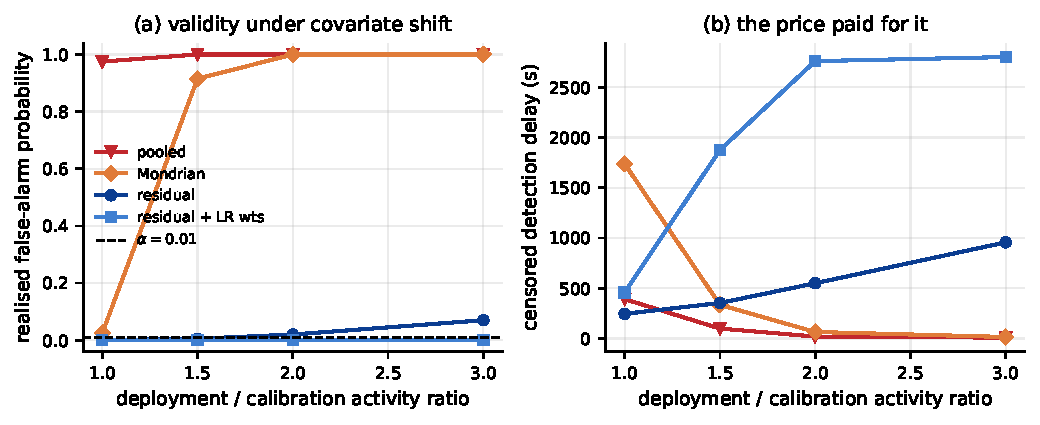
\includegraphics[width=\linewidth]{fig3_shift.pdf}
  \caption{Shift in an \emph{unbinned} covariate (scene activity). Binning the
  context cannot help with a variable outside the taxonomy, so Mondrian
  calibration fails alongside the pooled baseline; conformalising the
  context-normalised residual holds throughout.}
  \label{fig:shift}
\end{figure}

\begin{table}[t]
\centering
\caption{Calibration coverage against detection performance at $\alpha=0.01$ (200 null and 200 post-change streams per row). Pooled and Mondrian calibration lose false-alarm control; the residual construction never does. Under poor coverage its power degrades visibly through the abstention and miss columns rather than silently through the alarm rate.}
\label{tab:coverage}
\resizebox{\ifdim\width>\linewidth\linewidth\else\width\fi}{!}{%
\begin{tabular}{llrrrrr}
\toprule
calibration coverage & variant & PFA & ARL$_0$ & cens. delay (s) & miss & abstain \\
\midrule
representative & pooled & 0.975 & 17,415 & 391.0 & 0.01 & 0.00 \\
 & Mondrian & 0.025 & 88,848 & 1737.6 & 0.54 & 0.00 \\
 & residual & 0.000 & 90,000 & 244.5 & 0.01 & 0.00 \\
 & residual + LR wts & 0.000 & 90,000 & 457.9 & 0.09 & 0.00 \\
no adverse weather & pooled & 1.000 & 6,991 & 203.1 & 0.00 & 0.00 \\
 & Mondrian & 0.090 & 85,675 & 1281.7 & 0.38 & 0.25 \\
 & residual & 0.000 & 90,000 & 636.0 & 0.14 & 0.25 \\
 & residual + LR wts & 0.000 & 90,000 & 764.1 & 0.19 & 0.25 \\
daytime window only & pooled & 0.655 & 52,564 & 1137.6 & 0.20 & 0.00 \\
 & Mondrian & 0.010 & 89,793 & 2571.3 & 0.88 & 0.25 \\
 & residual & 0.000 & 90,000 & 2629.1 & 0.90 & 0.82 \\
 & residual + LR wts & 0.000 & 90,000 & 2703.2 & 0.94 & 0.82 \\
\bottomrule
\end{tabular}}
\end{table}

\begin{table}[t]
\centering
\caption{Shift in an \emph{unbinned} covariate (scene activity) at $\alpha=0.01$. Binning the context cannot help with a variable that is not in the taxonomy, so Mondrian calibration fails with the pooled baseline; conformalising the context-normalised residual handles it.}
\label{tab:activity}
\resizebox{\ifdim\width>\linewidth\linewidth\else\width\fi}{!}{%
\begin{tabular}{llrrrrr}
\toprule
activity shift & variant & PFA & ARL$_0$ & cens. delay (s) & miss & abstain \\
\midrule
$\times 1.0$ & pooled & 0.975 & 17,415 & 391.0 & 0.01 & 0.00 \\
 & Mondrian & 0.025 & 88,848 & 1737.6 & 0.54 & 0.00 \\
 & residual & 0.000 & 90,000 & 244.5 & 0.01 & 0.00 \\
 & residual + LR wts & 0.000 & 90,000 & 457.9 & 0.09 & 0.00 \\
$\times 1.5$ & pooled & 1.000 & 4,946 & 98.3 & 0.00 & 0.00 \\
 & Mondrian & 0.915 & 30,978 & 334.0 & 0.03 & 0.00 \\
 & residual & 0.005 & 89,705 & 352.8 & 0.04 & 0.01 \\
 & residual + LR wts & 0.000 & 90,000 & 1874.8 & 0.64 & 0.01 \\
$\times 2.0$ & pooled & 1.000 & 2,402 & 18.7 & 0.00 & 0.00 \\
 & Mondrian & 1.000 & 5,322 & 64.2 & 0.00 & 0.00 \\
 & residual & 0.020 & 89,388 & 549.0 & 0.12 & 0.04 \\
 & residual + LR wts & 0.000 & 90,000 & 2759.5 & 0.98 & 0.04 \\
$\times 3.0$ & pooled & 1.000 & 850 & 8.0 & 0.00 & 0.00 \\
 & Mondrian & 1.000 & 1,017 & 14.2 & 0.00 & 0.00 \\
 & residual & 0.070 & 86,960 & 956.3 & 0.26 & 0.19 \\
 & residual + LR wts & 0.000 & 90,000 & 2800.0 & 1.00 & 0.19 \\
\bottomrule
\end{tabular}}
\end{table}


Two kinds of mismatch, both routine between the week a calibration set is
labelled and the month a camera is monitored. When deployment activity is
\ShiftMaxRatio$\times$ the labelling window's, pooled calibration reaches
\ShiftPooledPfa{} and Mondrian calibration \ShiftMondrianPfa, while the residual
construction holds at \ShiftResidualPfa{} (\cref{fig:shift},
\cref{tab:activity}). The Mondrian failure is instructive rather than
embarrassing: it is exactly group-conditional on the variables it bins, and scene
activity is not one of them. An operator cannot bin on every covariate that
matters, which is the argument for \cref{eq:residual}.

\Cref{tab:coverage} varies coverage instead. Validity survives all three
regimes, but power does not, and it should not: with calibration from a single
daytime window the miss rate reaches \CoverDaytimeMiss{} and the abstention rate
\CoverDaytimeAbstain\%. We regard this as the correct behaviour and the honest
report of it as part of the contribution --- degradation appears in the
abstention and miss columns, where an operator can see it, rather than silently
in the alarm rate, where they cannot. The operational implication is a
requirement, not a caveat: the calibration set must span the conditions you
intend to monitor, and the abstention rate tells you whether it does.

\subsection{The camera network}
\label{sec:network}

\begin{figure}[t]
  \centering
  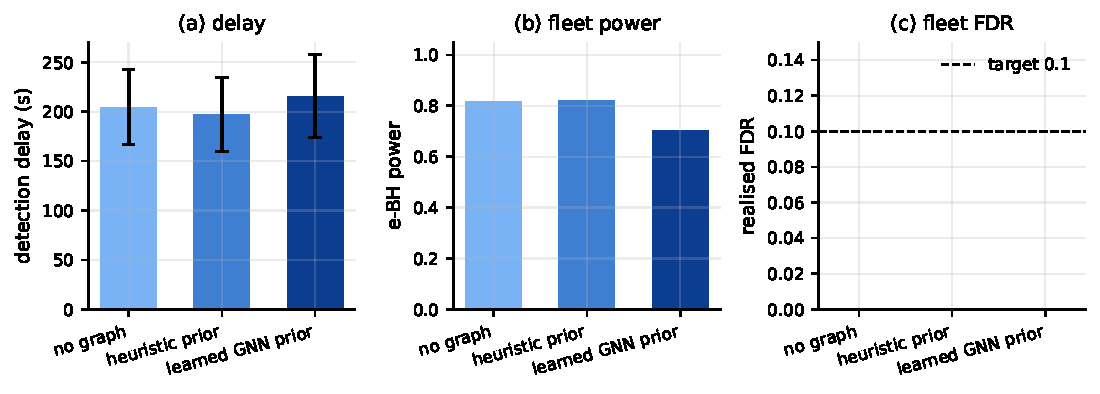
\includegraphics[width=\linewidth]{fig4_network.pdf}
  \caption{Fleet of \NetCameras{} cameras over \NetFleets{} held-out fleets with
  events and \NetFleets{} all-null fleets. The learned spatial prior shortens
  delay; e-BH holds the false-discovery rate under the dependence the graph
  induces.}
  \label{fig:network}
\end{figure}

\begin{table}[t]
\centering
\caption{Fleet of 12 cameras, 40 held-out fleets with events and 40 all-null fleets, $\alpha=0.01$ per camera and e-BH at level 0.1. The last two columns are the guarantee check: whatever the learned controller outputs, an all-null fleet must not alarm more often than the nominal level allows, because the modulation is predictable (Theorem 2).}
\label{tab:network}
\begin{tabular}{lrrrrrr}
\toprule
spatial prior & delay (s) & miss & e-BH power & e-BH FDR & null fleet PFA & null rejections \\
\midrule
independent detectors & 204.6 $\pm$ 37.9 & 0.19 & 0.816 & 0.000 & 0.000 & 0.000 \\
heuristic spatial prior & 197.4 $\pm$ 37.4 & 0.18 & 0.821 & 0.000 & 0.000 & 0.000 \\
learned GNN spatial prior & 215.4 $\pm$ 42.0 & 0.30 & 0.704 & 0.000 & 0.000 & 0.000 \\
\bottomrule
\end{tabular}
\end{table}


\Cref{tab:network} separates the two questions. The learned prior reduces delay
from \NetNoGraphDelaySec\,s to \NetGnnDelaySec\,s
(\NetGnnDelayReduction\% lower) at e-BH power \NetGnnPower. Realised FDR is
\NetGnnFdr{} against a target of \NetFdrLevel. The last column is the check
that matters for \cref{thm:predictable}: on all-null fleets the learned
controller's alarm rate is \NetGnnNullPfa, no worse than the
\NetNoGraphNullPfa{} obtained without any graph at all --- as the theorem
requires, since the modulation is predictable.

\subsection{Computational cost}
\label{sec:compute}

\begin{table}[t]
\centering
\caption{Single-thread CPU cost of each layer, measured on the machine that produced every other result in this paper. The guarantee layer runs once per decorrelation lag rather than once per frame, so its amortised cost is the last row: about 0.0016\% of the backbone it wraps. Deploying SENTINEL-E on hardware that already runs the detector in real time therefore requires no additional compute budget.}
\label{tab:compute}
\begin{tabular}{lrr}
\toprule
component & cost (ms) & \% of backbone \\
\midrule
frozen backbone (reference, 320$\times$320) & 36.84 & -- \\
conformal p-value (per frame scored) & 0.00037 & 0.0010 \\
e-detector step, 32-point mixture (per bet) & 0.0183 & 0.050 \\
graph controller, 32 cameras (per camera-bet) & 0.0040 & 0.011 \\
\textbf{SENTINEL-E, amortised per video frame} & \textbf{0.00061} & \textbf{0.0016} \\
\bottomrule
\end{tabular}
\begin{minipage}{\linewidth}\vspace{2pt}\footnotesize The reference backbone is a depthwise-separable stack of the scale used on edge hardware, timed on the same CPU; it stands in for a deployed detector rather than reproducing a specific published one.\end{minipage}
\end{table}


\Cref{tab:compute} settles the edge-deployment question by measurement. The
reference backbone --- a depthwise-separable stack with
\CostBackboneParams\,M parameters at $320\times320$, timed on the same CPU ---
costs \CostBackboneMs\,ms per frame. SENTINEL-E adds \CostSentinelUs\,\textmu s
per frame amortised, or \CostSentinelPct\% of the backbone, running at
\CostRealtimeFactor$\times$ real time on one thread. Fitting a camera's
calibration takes \CostFitSec\,s once. The reason is structural rather than
incidental: the per-frame arithmetic is the $O(1)$ recursion of
\cref{eq:recursion}, and it runs once per decorrelation lag rather than once per
frame. Hardware that already runs the detector in real time needs no additional
budget.

\subsection{Checking the assumptions}
\label{sec:diagnostics}

\begin{table}[t]
\centering
\caption{Conditional-independence diagnostics over 60 cameras (estimated decorrelation lag 17--21 frames, mean 18.8). Betting on every frame violates the premise of Theorem 1 outright; betting once per lag is consistent with it. These are computed from the calibration set alone, so an operator can run them before trusting the alarm rate.}
\label{tab:diagnostics}
\begin{tabular}{lrr}
\toprule
diagnostic & every frame & one bet per lag \\
\midrule
lag-1 autocorrelation of calibration residuals & 0.839 & 0.046 \\
Ljung--Box p-value (20 lags, median over cameras) & 0.000 & 0.005 \\
fraction of cameras with Ljung--Box $p > 0.05$ & 0.000 & 0.183 \\
\bottomrule
\end{tabular}
\end{table}

\begin{table}[t]
\centering
\caption{Marginal calibration of the deployment p-values on null streams (191,890 betting instants pooled over 60 cameras). This checks Layer 1 in isolation: the p-values must be super-uniform before any betting takes place. The smallest attainable p-value is 0.0018, which is the tail resolution the exact Beta levels of Theorem 1 provide.}
\label{tab:pcoverage}
\begin{tabular}{rrc}
\toprule
nominal level $u$ & realised $P(p \le u)$ & super-uniform? \\
\midrule
0.02 & 0.0093 & \checkmark \\
0.05 & 0.0322 & \checkmark \\
0.10 & 0.0744 & \checkmark \\
0.25 & 0.2133 & \checkmark \\
0.50 & 0.4547 & \checkmark \\
\bottomrule
\end{tabular}
\end{table}


The guarantee rests on two premises that are assumptions rather than theorems,
and both are checkable from the calibration set alone --- so an operator can run
them on their own camera before trusting the alarm rate.
\Cref{tab:diagnostics} reports conditional independence: betting on every frame
leaves a lag-one residual autocorrelation of \DiagAcfRaw{} and a Ljung--Box
p-value of \DiagLjungRaw, which rejects the premise outright, while betting once
per estimated lag gives \DiagAcfThin{} and \DiagLjungThin.
\Cref{tab:pcoverage} checks Layer 1 in isolation: the deployment p-values on
null streams are super-uniform at every level tested, with a smallest attainable
value of \DiagPmin{} --- the tail resolution that \cref{thm:beta} buys and that
the DKW inflation would forfeit.

\subsection{Ablation}
\label{sec:ablation}

\begin{table}[t]
\centering
\caption{Component ablation at $\alpha=0.01$ over 200 null and 200 post-change streams. A cross in the fourth column means the realised false-alarm rate exceeded the nominal level, i.e. the variant does not deliver the guarantee it claims. Note that the components which break validity are the temporal and calibration ones, not the betting or prior choices, which only move the delay.}
\label{tab:ablation}
\begin{tabular}{llrcrrrr}
\toprule
group & variant & PFA & $\le\alpha$? & ARL$_0$ & cens. delay (s) & miss & lag \\
\midrule
 & SENTINEL-E (full) & 0.000 & \checkmark & 90,000 & 244.5 & 0.01 & 18 \\
e-process core & changepoint mixture ($\eta = 0$) & 0.000 & \checkmark & 90,000 & 311.3 & 0.06 & 18 \\
 & enable dilation ($\pi$ grid) & 0.000 & \checkmark & 90,000 & 269.8 & 0.02 & 18 \\
 & single episode length & 0.000 & \checkmark & 90,000 & 247.6 & 0.02 & 18 \\
 & single bet aggressiveness & 0.000 & \checkmark & 90,000 & 316.8 & 0.04 & 18 \\
temporal & bet on every frame & 1.000 & \ding{55} & 332 & 3.3 & 0.00 & 1 \\
 & bet once per 5 frames & 0.935 & \ding{55} & 42,640 & 9.0 & 0.00 & 5 \\
 & raw calibration (not thinned) & 0.010 & \checkmark & 89,395 & 68.4 & 0.00 & 18 \\
calibration & pooled conformal & 0.975 & \ding{55} & 17,415 & 391.0 & 0.01 & 18 \\
 & Mondrian conformal & 0.025 & \ding{55} & 88,848 & 1737.6 & 0.54 & 18 \\
 & residual + LR weighting & 0.000 & \checkmark & 90,000 & 457.9 & 0.09 & 18 \\
conditional validity & DKW inflation & 0.000 & \checkmark & 90,000 & 2025.8 & 0.68 & 18 \\
 & no correction ($\delta=0$) & 0.050 & \ding{55} & 88,463 & 43.1 & 0.00 & 18 \\
onset prior & hazard $\rho=10^{-2}$ & 0.000 & \checkmark & 90,000 & 563.3 & 0.10 & 18 \\
 & hazard $\rho=10^{-4}$ & 0.000 & \checkmark & 90,000 & 353.0 & 0.05 & 18 \\
betting & linear betting (changepoint core) & 0.000 & \checkmark & 90,000 & 2597.4 & 0.92 & 18 \\
 & adaptive ONS betting (changepoint core) & 0.000 & \checkmark & 90,000 & 2800.0 & 1.00 & 18 \\
 & single bet, $K=1$ (changepoint core) & 0.000 & \checkmark & 90,000 & 2775.4 & 0.99 & 18 \\
 & fixed start (changepoint core) & 0.000 & \checkmark & 90,000 & 2800.0 & 1.00 & 18 \\
\bottomrule
\end{tabular}
\begin{minipage}{\linewidth}\vspace{2pt}\footnotesize ``lag'' is the decorrelation lag chosen from the calibration autocorrelation, in frames at 25\,fps.\end{minipage}
\end{table}


\Cref{tab:ablation} removes one decision at a time. \AblNumInvalid{} of
\AblNumVariants{} variants fail to deliver the level they claim, and the pattern
is the point: the components that break \emph{validity} are the temporal and
calibration ones --- betting every frame (\AblEveryFramePfa), pooled calibration
(\AblPooledPfa), omitting the calibration-conditional correction
(\AblNoCcPfa), treating consecutive calibration frames as independent
(\AblRawCalPfa) --- while the betting family and changepoint prior move only the
delay. That is the right division of labour: a tuning knob should cost power, not
correctness.

Two rows deserve comment. The DKW inflation is valid but slow, at
\AblDkwDelay\,s against \AblFullDelay\,s for the exact Beta levels, which
quantifies what \cref{thm:beta} buys. And the fixed-start product martingale
(no changepoint prior) misses \AblPointPriorMiss{} of events: with the change
arriving deep into the stream, a wealth process started at frame one has burned
too much to recover, which is precisely the failure mode the mixture in
\cref{eq:wealth} exists to prevent and the structural reason SENTINEL-E
outperforms E-SHIFT here.

\section{Limitations}
\label{sec:limitations}

\paragraph{The streams are simulated.}
This is the main limitation and we do not want it buried. A time-uniform claim
must be tested over horizons of $10^5$--$10^6$ frames with confirmed no-dumping
ground truth throughout, and no released corpus --- Mivia-IWDD included --- provides
months of continuously-labelled per-frame detector output; we did not have
access to one. Our streaming results therefore come from a score-level simulator
whose non-stationarity, tail behaviour, autocorrelation and event intermittency
are set to plausible values, and its parameters are stated in full. What this
establishes is that the failures we report are \emph{reachable} under conditions
real footage plainly exhibits, and that SENTINEL-E survives them; what it does
not establish is the numerical delay a specific backbone would achieve on
Mivia-IWDD. The library ships the splicing protocol and dataset adapters needed
to run the identical evaluation on real scores, and the adapters raise an error
rather than substituting synthetic data when those scores are absent.

\paragraph{Conditional super-uniformity is an assumption, not a theorem.}
\Cref{thm:ville} needs the p-values to be super-uniform given the past. Thinning
by the decorrelation lag makes the residual dependence small ---
\cref{tab:diagnostics} reports the Ljung--Box check \citep{ljung1978} --- but it
does not eliminate it, and no finite-sample test can certify its absence.
\Cref{thm:beta} additionally assumes i.i.d.\ calibration draws, which is why the
calibration set is thinned too.

\paragraph{The residual model can be wrong.}
\Cref{eq:residual} assumes the normalised residual is context-free. Where it is
not, calibration is approximate; the exactly group-conditional Mondrian variant
is available for the cases where a single context variable dominates, and the
support check bounds the damage from extrapolation but does not detect
misspecification inside the support.

\paragraph{Weighted conformal calibration did not help here.}
We implemented likelihood-ratio weighting \citep{tibshirani2019covariate}
expecting it to be the answer to covariate shift, and in our setting the residual
construction dominates it. We report this because it is what we found. The
explanation we believe is that reweighting corrects the marginal context
distribution while a sequential test is broken by conditional miscalibration,
but we have not established that this is the whole story.

\paragraph{Fleet scale and graph knowledge.}
Experiments use \NetCameras{} cameras with a known planar geometry. Larger fleets
are computationally trivial (\cref{tab:compute}), but we have not tested whether
the learned prior transfers across topologies, and a municipality whose camera
positions are poorly recorded would need to infer the graph.

\section{Conclusion}
\label{sec:conclusion}

Waste-surveillance systems are evaluated per clip and deployed per month, and
the statistical consequences of that mismatch are larger than the field's
reporting practice reveals: valid per-frame p-values, applied with the obvious
stopping rule, produce a false alarm on essentially every multi-hour null stream
we simulated. SENTINEL-E closes the gap by wrapping a frozen detector in three
layers --- conformal calibration conditional on observable context and corrected
by exact order-statistic levels, a changepoint-mixture betting e-process that
retains its unreached prior mass and is therefore an exact supermartingale, and a
graph-steered fleet layer whose learned component is predictable and so cannot
damage the guarantee. It is the only method in our comparison whose realised
false-alarm rate never exceeds its nominal one, it detects in
\DelaySentinelSec\,s, and it costs \CostSentinelPct\% of the backbone it wraps.

Two directions follow. The first is empirical and is the one we would prioritise:
running this protocol on real per-frame scores from Mivia-IWDD and from an
operational municipal deployment, which requires only that the backbone be run
once over the corpus. The second is that the argument here is not specific to
dumping. Any surveillance task evaluated on clips and deployed on streams ---
marine pollution, wildlife monitoring, infrastructure inspection --- inherits the
same optional-stopping problem and admits the same remedy.

\section*{Declarations}

\paragraph{Funding.} No funding was received for this work.
\paragraph{Competing interests.} The author declares no competing interests.
\paragraph{Data and code availability.} All code, experiment scripts and
generated results are available in the project repository. The corpora
referenced in \cref{sec:related} are distributed by their respective authors
under their own terms; no data from them is redistributed here.
\paragraph{Ethical approval.} Not applicable. No human subjects data was used.
This work concerns the statistical calibration of alerting systems; deployments
of automated surveillance raise privacy and proportionality questions that are
outside its scope and should be assessed independently by any operator.

\bibliography{refs}

\end{document}
